\chapter{Spinning Neutron Stars in Mixed Binaries}

\section{Chapter Overview}

An Overview of my chapter here.

\section{Chapter TDL}
\begin{itemize}
\item Previous work on mixed binaries with spinning stars?
\item Plot of omega vs chi for NS spin
\item 3d parameter space plot
\item Information about how easy/difficult it is to do the solution?
  Number of gridpoints, constraints, its?
\item Geoffrey massive disk formation 
\item Do the high $\omega$ curves go to higher lev than 8?
\end{itemize}


\section{Papers to read}

Insert here

%\section{Post-Intro}
%\red{What are all the items I need post-intro}

%\begin{itemize}
%\item What is the code we use?
%\item  How does it work?
%\item What is the domain? What does it look like?
%\item What is the resolution of the domain? How is it chosen?
%\item Finite difference grid? Resolution?
%\item Domain symmetries
%%\item What equations are we solving?
%\item Equilibrium assumption
%\item Values of $\Omega$ and $v_r$




%\end{itemize}


\section{Introduction}

%\red{Topics to cover in intro}
%\begin{enumerate}
%\item X
%\item XX
%\end{enumerate}

Black hole - neutron stars (BH-NS) inspirals and mergers are an important potential source of gravitaitonal waves for ground-based detectors like Advanced LIGO and Virgo. Information abou tthe inspiral can help determine the neutron star equation of state. Electromagnetic signals from the merger can give clues about the violent physical processes that occur. Gravitaitonal waves help test general relativity in the genuinely non-linear regime.

The parameter space of Bh-ns binaries is quite rich. The mass ratio, $q$, and black hole spin, $\vec{\chi}$, have been of particular interest in numerical simulations. Foucart \red{cite} gave an analytic description of how this combination can predict the time of neutron star disruption. The neutron star equation of state is also of great interest. The size of the star is directly lninked ot when tidla disruption occurs. One aspect that has not been studied, however, is the effect of neutron star spin. All simulations to date use irrotational neutron star in their Bh-NS binaries. Since no Bh-NS binaries have been directly observed, the NS spins are, at least observationally, unconstrained. Spinning NS will affect the gravitational waveforms and cause the inspiral to proceed more slowly (for spin-aligned NS). \red{cite} XX found that NS spins of XX in Bh-ns binaries could cause Advanced LIGO to miss XX percent of potential signals. The spin could also affect the time of NS disruption, as the stellar material will be less tightly bound to the stellar surface.

Recently, \cite{Tacik:2015tja} used the {\tt SpEC} code to create and
evolve initial data sets of binary neutron star systems with arbitrary
spins. In this chapter, we extend this code to create initial data for
Bh-ns systems where the NS spin is arbitrary. The structure of this
chapter is as follows: In section XX, we review the formalism
developed in \cite{Tichy:2011gw} to create binaries with spinning NS,
and discuss how this is extended to Bh-NS systems. In section XX we
present data demonstrating the robustness and convergence of this
initial data. Finally, we conclude the chapter in section XX.

\section{Initial Data Formalism}
In this section we will discuss the formalism used to solve the
Einstein field equations and create quasi-equilibrium initial data for
BH-NS binaries with spinning neutron
stars. We begin with the $3+1$ decomposition of the space-time metric
tensor,
\begin{equation}
g_{\mu\nu}dx^{\mu}dx^{\nu} = -\alpha^2dt^2 + \gamma_{ij}\left(dx^i +
  \beta^idt\right)\left(dx^j+\beta^jdt\right),
\end{equation}
where $\alpha$ is the lapse function, $\beta^i$ is the shift vector,
and $\gamma_{ij}$ is the induced metric on a spatial hypersurface
$\Sigma(t)$. The normal vector $n^{\mu}$ to $\Sigma(t)$ is related to
the coordinate time $t$ by
\begin{equation}
t^{\mu} = \alpha n^{\mu} + \beta^{\mu}.
\end{equation}
The extrinsic curvature of $\Sigma(t)$ is given by
\begin{equation}
K_{\mu\nu} = -\frac{1}{2}\mathcal{L}_n\gamma_{\mu\nu},
\end{equation}
where $\gamma_{\mu\nu}=g_{\mu\nu}+n_{\mu}n_{\nu}.$ and $\mathcal{L}_n$
is the Lie derivative in the direction of the $n^{\mu}$. We restrict our
attention to the spatial part of the extrinsic curvature, $K^{ij}$,
since $n_{\mu}K^{\mu\nu}=0$ by construction. It is convenient to
decmopose it into its trace and trace-free parts,
\begin{equation}
K^{ij} = A^{ij}+\frac{1}{3}K\gamma_{ij}.
\end{equation}
The matter in the system is modelled with the stress-energy tensor of
a perfect fluid 
\begin{equation}
T_{\mu\nu}=\left(\rho+P\right)u_{\mu}u_{\nu}+Pg_{\mu\nu},
\end{equation}
where $\rho$ is the fluid's energy density, $P$ is its pressure, and
$u^{\mu}$ is its four-velocity. It is further useful to define the
projections of the matter quantities,
\begin{eqnarray}
E &=& T^{\mu\nu}n_{\mu}n_{\nu},\\
S &=& \gamma^{ij}\gamma_{i\mu}\gamma_{j\nu}T^{\mu\nu}, \\
J^i &=& -\gamma^{i}_{\mu}T^{\mu\nu}n_{\nu}.
\end{eqnarray}
The spatial metric is decomposed with the conformal transformation
\begin{equation}
\gamma_{ij}=\Psi^4\tilde{\gamma}_{ij},
\end{equation}
where $\Psi$ is called the conformal factor, and $\tilde{\gamma}_{ij}$
is the conformal metric. The other quantities in the initial value
problem use the following conformal transformations:
\begin{eqnarray}
E &=& \Psi^{-6}\tilde{E}, \\
S &=& \Psi^{-6}\tilde{S}, \\
J^i &=& \Psi^{-6}\tilde{J}^i, \\
A^{ij} &=& \Psi^{-10}\tilde{A}^{ij}, \\
\alpha &=& \Psi^{6}\tilde{\alpha}. 
\end{eqnarray}
$\tilde{A}^{ij}$ is related to the shift and to the time derivative of
the conformal metric, $\tilde{u}_{ij}=\partial_t\tilde{\gamma}_{ij}$,
by
\begin{equation}
\tilde{A}^{ij} =
\frac{1}{2\tilde{\alpha}}\left[\left(\tilde{\mathrm{L}}\beta\right)^{ij}-\tilde{u}^{ij}\right],
\end{equation}
where $\tilde{L}$ is the conformal longitudinal operator,
\begin{equation}
\left(\tilde{L}V\right)^{ij}=\tilde{\nabla}^iV^j + \tilde{\nabla}^jV^i
- \frac{2}{3}\tilde{\gamma}^{ij}\tilde{\nabla}_kV^k.
\end{equation}
We solve the extended conformal thin sandwich (XCTS) equations, which are a set of 5
coupled non-linear equations.
\begin{eqnarray}
2\tilde{\alpha}\bigg[\tilde{\nabla}_j\left(\frac{1}{2\tilde{\alpha}}\big(\tilde{L}\beta\big)^{ij}\right)-\tilde{\nabla}_j\left(\frac{1}{2\tilde{\alpha}}\tilde{u}^{ij}\right) && \nonumber\\
\label{eq:XCTS-Shift}
-\frac{2}{3}\Psi^6\tilde{\nabla}^iK-8\pi\Psi^4\tilde{J}^i\bigg] &=&0,
\end{eqnarray}

\begin{eqnarray}
\tilde{\nabla}^2\Psi - \frac{1}{8}\Psi\tilde{R} -
\frac{1}{12}\Psi^5K^2  \qquad\quad && \nonumber \\
\label{eq:XCTS-ConformalFactor}
+\frac{1}{8}\Psi^{-7}\tilde{A}_{ij}\tilde{A}^{ij} +
2\pi\Psi^{-1}\tilde{E} &=& 0,
\end{eqnarray}

\begin{eqnarray}
&&\tilde{\nabla}^2\left(\tilde{\alpha}\Psi^7\right) -
\left(\tilde{\alpha}\Psi^7\right)\bigg[\frac{1}{8}\tilde{R}+\frac{5}{12}\Psi^4K^2+\frac{7}{8}\Psi^{-8}\tilde{A}_{ij}\tilde{A}^{ij}\nonumber \\
\label{eq:XCTS-Lapse}
&&+2\pi\Psi^{-2}\big(\tilde{E}+2\tilde{S}\big)\bigg]=-\Psi^5\left(\partial_{t}K
- \beta^{k}\partial_kK\right).
\end{eqnarray}
These are solved
for the conformal factor, $\Psi$, the densitized lapse, $\alpha\Psi$,
and the shift, $\beta^i$.

The matter content of $\Sigma(t)$ is determined by $\tilde{E}$,
$\tilde{S}$, and $\tilde{J}^i$. The free data are $\gamma_{ij}$,
$\tilde{u}_{ij}$, $K$ and $\partial_t K$. $\tilde{u}_{ij}=0$ and
$\partial_t K=0$ are natural choices in a coordinate system corotating
with the binary. The
choice of the conformal metric will be discussed in section~\ref{sec:NumMethods}.

Let us now further discuss the matter content of the neutron star. The
energy density of the fluid is $\rho=\rho_0\left(1+\epsilon\right)$,
where $\rho_0$ is the baryon density and $\epsilon$ is the internal
energy. The specific enthalpy of the fluid is
\begin{equation}
h=1+\epsilon+\frac{P}{\rho_0}.
\end{equation}
It is convenient to introduce the following projections of the four
velocity:
\begin{eqnarray}
\gamma &=& \gamma_n\gamma_0\left(1-\gamma_{ij}U^iU^j_0\right), \\
\gamma_0 &=& \left(1 - \gamma_{ij}U^i_0U^j_0\right)^{-1/2}, \\
\gamma_n &=& \left(1 - \gamma_{ij}U^iU^j\right)^{-1/2}, \\
U^i_0 &=& \frac{\beta^i}{\alpha}, \\
u^{\mu} &=& \gamma_n\left(n^u+U^\mu\right), \\
U^{\mu}n_{\mu}&=&0.
\end{eqnarray}
Following \cite{Tichy:2011gw}, the three-velocity is written as the sum
of an irrotational part (the gradient of a potential $\phi$) and a
rotational part $W$:
\begin{equation}
U^i =
\frac{\Psi^{-4}\tilde{\gamma}^{ij}}{h\gamma_n}\left(\partial_j\phi+W_j\right).
\end{equation}
$W$ is a freely chosen vector in this formalism; we will discuss this choice in section~\ref{sec:NumMethods}.

The matter fluid must satisfy the continuity equation and the Euler equation. The continuity equation is a second order elliptic equation for the potential $\phi$:
\begin{equation}
\frac{\rho_0}{h}\nabla^{\mu}\nabla_{\mu}\phi+\left(\nabla^{\mu}\phi\right)\nabla_{\mu}\frac{\rho_0}{h}=0.
\end{equation}
Under the assumptions made in \cite{Tichy:2011gw}, this equation can be written as
\begin{align}
\rho_0\,\bigg\{\!\!&-\tilde{\gamma}^{ij}\partial_i\big(\partial_j\phi+W_j\big)  + \frac{h\beta^i\Psi^4}{\alpha}\partial_i\gamma_n + hK\gamma_n\Psi^4 \nonumber\\
&\qquad+\Big[\tilde{\gamma}^{ij}\tilde{\Gamma}^k_{ij}+\gamma^{ik}\partial_i\big(\ln \frac{h}{\alpha\Psi^2}\big)\Big] 
\big(\partial_k\phi+W_k\big) \bigg\} \nonumber \\
&=\tilde{\gamma}^{ij}\big(\partial_i\phi+W_i\big)\partial_j\rho_0 - \frac{h\gamma_n\beta^i\Psi^4}{\alpha}\partial_i\rho_0.
\label{eq:Continuity}
\end{align}
The Euler equation is solved for the specific enthalpy $h$. The
solution is, as shown in \cite{Tichy:2011gw}:
\begin{equation}
h = \sqrt{L^2 -
  \left(\nabla_i\phi+W_i\right)\left(\nabla^i\phi+W^i\right)},
\end{equation}
where
\begin{equation}
L^2 =
\frac{b+\sqrt{b^2-4\alpha^4\left(\left(\nabla_i\phi+W_i\right)W^i\right)^2}}{2\alpha^2},
\end{equation}
and
\begin{equation}
b =
\left(\beta^i\nabla_i\phi+C\right)^2+2\alpha^2\left(\nabla_i\phi+W_i\right)W^i.
\end{equation}

The boundary condition at the surface of the neutron star can deduced from the $\rho_0\rightarrow 0$ limit of the continuity equation:
\begin{equation}
\tilde{\gamma}^{ij}\left(\partial_i\phi+W_i\right)\partial_j\rho_0=\frac{h\gamma_n\beta^i\Psi^4}{\alpha}\partial_i\rho_0.
\end{equation}
The boundary condition at infinity (which is in practice, in our computational grid, at $R=10^{10}$) are the requirement of a Minkowski metric in the intertial frame:
\begin{eqnarray}
\beta^i&=&0,\\
\alpha\Psi &=& 1,\\
\Psi &=&1.
\end{eqnarray}
The interior of the black hole is excised from the computation domain. The boundary conditions at the surface of the black hole horizon are~(\cite{Cook2004}):
\begin{eqnarray}
\label{eq:BhBoundary}
\tilde{s}^k\nabla_k\log\Psi&=&-\frac{1}{4}\left(\tilde{h}^{ij}\tilde{\nabla}^i\tilde{s}_j-\Psi^2h^{ij}K_{ij}\right) \\
\label{eq:BhBoundary2}
\beta_{\perp}&=&\alpha \\
\label{eq:BhBoundary3}
\beta_{\parallel}&=&\Omega_{j}^{BH}x_k\epsilon^{ijk}
\end{eqnarray}
whre $s$ is the outward pointing unit normal to the apparent horizon
surface, $h^{ij}$ is the 2-metric on the surface, and $\Omega^{BH}$ is a
free parameter that determines the spin of the black hole.

The force balance equation at the centre of the NS is 
\begin{equation}
\nabla\log h=0.
\end{equation}
We can re-write this equaiton as 
 \begin{equation}
\label{eq:OmegaDriver}
\nabla\ln\left(\alpha^2-\gamma_{ij}\beta^{i}\beta^{j}\right)=-2\nabla\ln\Gamma,
\end{equation}
where
\begin{equation}
\Gamma
=\frac{\gamma_n\left(1-\left(\beta^i+\frac{W^i\alpha}{h\gamma_n}\right)\frac{\nabla_i\phi}{\alpha
    h\gamma_n}- \frac{W_i W^i}{\alpha^2\gamma_n^2}\right) } { \sqrt{ 1
    - \left(\frac{\beta^i}{\alpha}+\frac{W^i}{h\gamma_n}\right)
    \left(\frac{\beta_i}{\alpha}+\frac{W_i}{h\gamma_n}\right) } } ,
\end{equation}
which is a second order equation for the orbital
frequency $\Omega$. If desired, this equation can be solved to find a
best guess for the orbital frequency. Alternatively, eccentricity
removal techniques, such as those used in \cite{Tacik:2015tja} can be
used to find the best value of the orbital frequency.

$W$ is chosen as as to give the NS a uniform rotational
profile. Following our work in \cite{Tacik:2015tja}, we use
\begin{equation}
W^i=\epsilon^{ijk}\omega^jr^k,
\end{equation}
where $\epsilon^{ijk}=\{\pm1,0\}$, $r^k$ is the position vector relative to the centre of the star, and $\omega^j$ is a freely chosen constant vector.

The angular momentum of the black hole is computed as 
\begin{equation}
\label{eq:BhSpin}
S=\frac{1}{8\pi}\oint_{\mathcal{H}}\phi^is^jK_{ij}dA
\end{equation}
where $\mathcal{H}$ is the black hole's apparent horizon, $s^j$ is the
outward-pointing unit-normal and $\phi^i$ is an azimuthal vector
field. The dimensionless spin is defined as
\begin{equation}
\chi=\frac{S}{M^2}
\end{equation}
where $M$ is the Christodoulou mass
\begin{equation}
M^2=M_{\rm irr}^2+\frac{S^2}{4M_{\rm irr}^2}.
\end{equation}
The irreducible mass is related to the surface area of the horizon
\begin{equation}
M_{\rm irr}=\sqrt{A/16\pi}.
\end{equation}
Following the method introduced in \cite{Tacik:2015tja} we also compute the dimensionless spin
of the neutron star in the same way, normalizing it by its
Arnowitt-Deser-Misner (ADM) mass.

\section{Numerical Methods}
\label{sec:NumMethods}
Let us now discuss how we solve these ellitpic equations. We use the
pseduo-spectral multi-grid elliptic solver developed in
\cite{Pfeiffer2003} and enhanced in \cite{FoucartEtAl:2008} to incorporate matter. The computational domain is divided into a number of subdomains. A small cube is placed at the centre of the NS. Overlapping this cube is a spherical shell whose outer boundary deforms to fit the NS surface. These are surrounded by an additional spherical shell. The black hole is represented by two concentric spherical shells. Their inner bounday is required to be an apparent horizon. Three rectangular parallelpipeds surround the axis passing through the centres of the BH and the NS - one between them and one on each side of the objects. An additional eight cylindrical shells are placed around the same axis to cover the intermediate field region. The far-field region is covered by a large spherical shell whose outer boundary is placed at $R=10^{10}$ using an inverse radial mapping. This domain is visualized in Fig.~\ref{fig:BhNsDomain}.

\begin{center}
\begin{figure}[!ht]
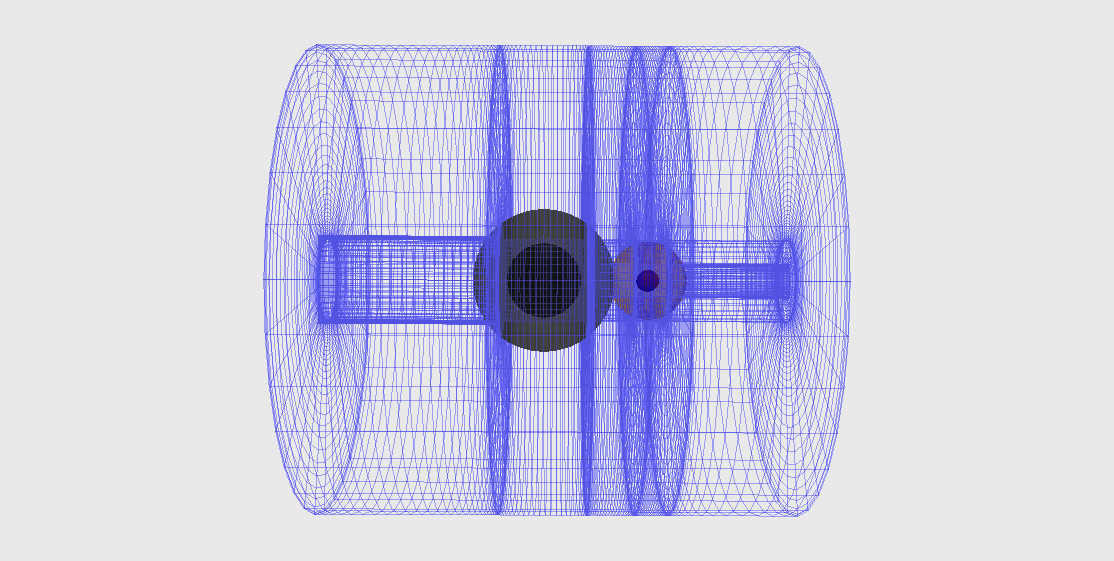
\includegraphics[scale=0.45]{chap4/BhNsDomain.png}
\caption[Visualization of the Bh-Ns domain
decomposition.]{Visualization of the Bh-Ns domain decomposition. The
  black object on the left is the black hole and the orange object on
  the right is the neutron star. The blue wireframes represent the
  various cylinders and rectangular parallelpipeds in the
  domain. \red{[Make this look nicer]}}
\label{fig:BhNsDomain}

\end{figure}
\end{center}

All variables (metric and hydrodynamical) are decomposed on sets of
basis functions on each subdomain. Finite difference schemes are
needed for hydrodynamical quantities during evolutions so as to
capture shocks, but for initial data, where shocks are not present, spectral methods are suitable and exponentical convergence can be guaranteed. The resolution of each domain is synonymous with the number of colocation points used. The resolution of each domain is chosen by hand at the start of the initial data solve, and then modified several times using an adaptive scheme. To discuss the resolution of the computational domain for the purpose of convergence tests, we will use the notation
\begin{equation}
N^{1/3}=\left(\sum N_i\right)^{1/3},
\end{equation}
where we are summing the colocation points of all of the
subdomains. This gives an indication of the average resolution in each
diredction.A typical initial data solve might start with, using example numbers, $N^{1/3}\sim 33$ and end with $N^{1/3}\sim 80$

Construction of initial data begins by choosing values for the free parameters in the problem. In particular, these are
\begin{itemize}
\item The black hole mass, $M_{\rm BH}$.
\item The black hole's target dimensionless spin vector, $\vec{\chi_{\rm BH}}$.
\item The neutron star's baryon mass, $M_{b}$.
\item The neutron star's equation of state, .
\item The neutron star's spin vector, $\omega^i$.
\item The separation between the centres of the BH and NS, $D$.
\item The orbital angular velocity, $\Omega_0$.
\item The initial infall velocity parameter, $\dot{a}$
.
\end{itemize}
Additionally, perscription is required for the free
metric variables, $\tilde{g}_{ij}$ and $K$. We use the following: near the black hole they
are equal to the values for a black hole with the same spin and boost
velocity,
written in Kerr-Schild coordinates. Near the neutron star, they are a
conformally flat metric and $K=0$. They fall-off from the black hole
to the neutron star with a function of the form $e^{(-r/w)^4}$, where
$w$ is half the coordinate separation between them.

Let's now discuss the algorithm we use to solve for the initial data. 

\begin{enumerate}
\item If on the first resolution step, set $\omega^i=0$, otherwise set
  to the desired value. This has been found to help with overall convergence. Additionally, impose a maximum radius out to which to apply $W^i=\epsilon^{ijk}\omega^jr^k$, otherwise low density material at high radius can lead to superluminal velocities.

\item Solve the non-linear XCTS equations for the metric variables
  $X=\left(\beta^i,\Psi,\alpha\Psi\right)$ assuming the matter source
  terms are fixed. Update the metric variables using a relaxation
  scheme
\begin{equation}
X^{n+1}=\lambda X^{*} + (1-\lambda)X^n,
\end{equation}
where $X^{*}$ is the result found by solving the XCTS equations, and $X^{n}$ is
the previous value of $X$.
We use $\lambda=0.3$.

\item Impose equatorial symmetry. This should only be done if both the
  NS and the BH have no spin components in the plane. But if it can be
  imposed, it will speed convergence.

\item Locate the surface of the star. The surface of the star is
  reprsented in terms of spherical harmonics
\begin{equation}
R(\theta,\phi)=\sum c_{lm}Y^{lm}(\theta,\phi)
,
\end{equation}
and for a polytropic equation of state, the surface
should satisfy $h(R(\theta,\phi)=1$. 

\item Compute the ADM linear momentum $P_{\rm ADM}$, as 
\begin{equation}
P_{\rm ADM}^i = \frac{1}{8\pi}\oint_{S_{\infty}}K^{ij}dS_j.
\end{equation}
If its norm has changed by less than 10\% in the last iteration, move
the centre of the BH so as to zero-out the momentum of the
system. Additionally, modify the radius of the excision surface to
drive $M_{\rm BH}$ to the desired value.

\item If desired, adjust the orbital angular frequency using Eq.~\ref{eq:OmegaDriver}.

\item Get the spin of the BH by evaluating Eq.~\ref{eq:BhSpin}. Then
  modify the parameter $\Omega$ in Eq.~\ref{eq:BhBoundary} to drive
  the black hole spin to the target value.

\item Fix the Euler constant by evaluating the integral
\begin{equation}
M_{B}=\int \rho_0\Psi^6\gamma_ndV
\end{equation}
as a function of the Euler
constant, and using the secant method to drive the baryon mass to the
desired value.

\item Solve the elliptic equations for the velocity potential, $\phi$,
  and update using the same relaxation scheme as described above.

\item Are all equations satisfied to the desired accuracy? If no, go
  to step two, otherwise proceed.

\item Compute the truncation error for the current solution by
  examining the spectral coefficients of the metric variables. If the
  truncation error is too large, adjust the number of grid points and
  return to step 1.

\end{enumerate}

\section{Results}

%\subsection{bla}
%In this section we will demonstrate that we are able to construct robust initial data for generic bh-ns binaries with a spinning neutron star. To begin, we will focus on two axes of the mutli-dimensional parameter space - mass ratio and black-hole spin - while keeping the NS parameters fixed. In particular, we use a neutron star wtih ADM mass, $M_{\rm ADM}=1.4M_{\odot}$, equation of state $P=\kappa\rho_0^\Gamma\left(\Gamma=2.0, \kappa=101.45\right)$ and spin parameter, $\vec{\omega_{\rm NS}}=0.017\hat{z}$, corresponding to a dimensionless spin $\vec{\chi_{\rm NS}}\sim0.4\hat{z}$. The black hole is given a mass, $M_{\rm BH}=qM_{\rm ADM}$ and a dimensionless spin $\vec{\chi_{\rm BH}}=\chi\hat{z}$. In the first initial data sqeuence, we keep $q=7$ fixed, and vary $q=\{0,0.1,0.2,0.3,0.4,0.5,0.6,0.7,0.8,0.9,0.95\}$. In the second initial data sequence, we keep $\chi=0.9$ fixed and vary $q=\{2,3,4,5,6,7,8,9,10\}$. In each case, the BH and the NS are separated by a coordinate distance $D=7.44\left(M_{\rm BH}+M_{\rm ADM}\right)=7.44M$, and have an initial orbital angular velocity $M\Omega_{\rm orb}=0.0413$, with no additional infall velocity ($\dot{a}=0$). We will now focus on a subset of these initial data sets to demonstrate initial data convergence. In particular, the sets with $q=3$, $q=5$, $q=10$, $\chi=0$, $\chi=0.5$, $\chi=0.95$.



\subsection{Initial Data Set Parameters}
Let us begin by discussing the parameters for the initial data sets to be discussed in this work. As a starting point, we use the six BH-NS configurations described in Table 1 of \cite{Foucart:2013a}. All binaries have a mass ratio $q=7$ and a black hole spin magnitude of $\chi_{\rm BH}=0.9$. The neutron star in each binary has an ADM mass of $1.4M_{\odot}$. In practice, this means that is fixed to have the same baryon mass as that of an isolated, non-spinning neutron star with ADM mass $1.4M_{\odot}$. There are three different NS equations of state used. They are all polytropic equations of state ($P=\kappa\rho^\Gamma$) with $\Gamma=2$, but vary in terms of $\kappa$, resulting in different neutron star compactnesses. The values of $\kappa$ used are $84.28$, $92.12$, $101.45$, which result in compactnesses, respectively, of $0.170$, $0.156$, $0.144$, for non-spinning neutron stars with ADM Mass $1.4M_{\odot}$. We will use the notation $R12$, $R13$ and $R14$ to refer to these configurations, respectively. The $R12$ and $R13$ configurations are only set with the black hole spin aligned with the orbital angular momentum. For $R14$, we also create data sets with the black hole spin misaligned by $20^{\circ}$, $40^{\circ}$ and $60^{\circ}$. The non-parallel part of the black hole spin is set parallel to the $\hat{x}$ axis. In each case the initial separation between the black hole and the neutron star is $D=7.44M$. The initial infall velocity parameter $\dot{a}$ is set to $0$. The orbital angular velocity is the same as in \cite{Foucart:2013a} and is indicated in table~\ref{tab:FullBHNSParameters}.

The above constitutes 6 different configurations. For each of these 6
configurations, we choose an additional 6 configurations of neutron
star spins (thus 36 total configurations). In particular we choose
three directions - aligned with the orbital angular momentum,
anti-aligned with the orbital angular momentum, and completley in the
orbital plane, parallel to the $\hat{x}$ direction. For each of these
3 directions, we use a ``high-spin'' and a ``low-spin''. These are
typically $\chi_{NS}\sim 0.4$ and $\chi_{\rm NS}\sim 0.1$,
respectively. In our naming notation, we use a large arrow
($\Uparrow$)  for the ``high-spin'' configurations and a small arrow
($\uparrow$) for the ``low-spin'', with the direction of the arrow
indicating the direction of the NS spin vector. The full parameters of
the initial data sets are summarized in Table
~\ref{tab:FullBHNSParameters}. In particular, the name of the run using the naming convention discussed,
the black hole spin direction, the baryon mass of the neutron star, the orbital angular velocity of the system,
the approximate number of orbits before merger, the neutron star spin vector $\vec{\omega}$, and the measured dimensionless
spin of the neutron star. Note that the number of orbits is taken from \cite{Foucart:2013a}, and doesn't account for the neutron star
spin. Note also since "merger" is defined by the maximum amplitude of the gravitaitonal waveform, this quantity isn't perfectly well-defined
for precessing binaries.

\begin{longtable}{l|c|c|c|c|c|c}
\centering
%\begin{tabular}{l|c|c|c|c|c|c}
Name & $\Theta_{\rm BH}$ & $M^b_{\rm NS}$ & $M\Omega_{\rm orbit}$ & $\sim N_{\rm orb}$ & $\vec{\omega_{\rm NS}}$ & $\vec{\chi_{\rm NS}}$  
\\\hline
{\tt R12i0$\uparrow$}&$0^\circ$ & 1.5212 & 0.0413 & 10.25 & $0.00667\hat{z}$ & $0.0995\hat{z}$ \\
{\tt R12i0$\Uparrow$}&$0^\circ$ & 1.5212 & 0.0413 & 10.25 & $0.0225\hat{z}$ & $0.4093\hat{z}$ \\
{\tt R12i0$\downarrow$}&$0^\circ$ & 1.5212 & 0.0413 & 10.25 & $-0.00667\hat{z}$& $-0.0895\hat{z}$\\
{\tt R12i0$\Downarrow$}&$0^\circ$ & 1.5212 & 0.0413 & 10.25 & $-0.0225\hat{z}$ & $-0.4030\hat{z}$ \\
{\tt R12i0$\rightarrow$}&$0^\circ$ & 1.5212 & 0.0413 & 10.25 & $0.00667\hat{x}$ & $0.0936\hat{x}$\\
{\tt R12i0$\Rightarrow$}&$0^\circ$ & 1.5212 & 0.0413 & 10.25 & $0.0225\hat{x}$ & $0.3989\hat{x}$ \\
\hline
{\tt R13i0$\uparrow$}&$0^\circ$ & 1.5128 & 0.0413  & 10.15 & $0.00555\hat{z}$ & $0.0997\hat{z}$ \\
{\tt R13i0$\Uparrow$}&$0^\circ$ & 1.5128 & 0.0413 & 10.15 & $0.019\hat{z}$ & $0.3911\hat{z}$ \\
{\tt R13i0$\downarrow$}&$0^\circ$ & 1.5128 & 0.0413 & 10.15 & $-0.00555\hat{z}$& $-0.0845\hat{z}$\\
{\tt R13i0$\Downarrow$}&$0^\circ$ & 1.5128 & 0.0413 & 10.15 & -$0.019\hat{z}$ & $-0.3793\hat{z}$ \\
{\tt R13i0$\rightarrow$}&$0^\circ$ & 1.5128 & 0.0413 & 10.15 & $0.00555\hat{x}$ & $0.0913\hat{x}$\\
{\tt R13i0$\Rightarrow$}&$0^\circ$ & 1.5128 & 0.0413 & 10.15 & $0.019\hat{x}$ & $0.3771\hat{x}$ \\
\hline
{\tt R14i0$\uparrow$}&$0^\circ$ & 1.5049 & 0.0413 & 9.85 & $0.005541\hat{z}$ & $0.1188\hat{z}$ \\
{\tt R14i0$\Uparrow$}&$0^\circ$ & 1.5049 & 0.0413 & 9.85 & $0.017\hat{z}$ & $0.4109\hat{z}$ \\
{\tt R14i0$\downarrow$}&$0^\circ$ & 1.5049 & 0.0413 & 9.85 & $-0.005541\hat{z}$& $-0.0965\hat{z}$\\
{\tt R14i0$\Downarrow$}&$0^\circ$ & 1.5049 & 0.0413 & 9.85 & -$0.017\hat{z}$ & $-0.3915\hat{z}$\\
{\tt R14i0$\rightarrow$}&$0^\circ$ & 1.5049 & 0.0413 & 9.85 & $0.005541\hat{x}$ & $0.1066\hat{x}$\\
{\tt R14i0$\Rightarrow$}&$0^\circ$ & 1.5049 & 0.0413 & 9.85 & $0.017\hat{x}$ & $0.3907\hat{x}$ \\
\hline
{\tt R14i20$\uparrow$}&$20^\circ$ & 1.5049 & 0.0412 & 9 & $0.005541\hat{z}$ & $0.1188\hat{z}$ \\
{\tt R14i20$\Uparrow$}&$20^\circ$ & 1.5049 & 0.0412 & 9 & $0.017\hat{z}$ & $0.4110\hat{z}$ \\
{\tt R14i20$\downarrow$}&$20^\circ$ & 1.5049 & 0.0412 & 9 &  $-0.005541\hat{z}$& $-0.0964\hat{z}$\\
{\tt R14i20$\Downarrow$}&$20^\circ$ & 1.5049 & 0.0412 & 9 & -$0.017\hat{z}$ & $-0.3915\hat{z}$ \\
{\tt R14i20$\rightarrow$}&$20^\circ$ & 1.5049 & 0.0412 & 9 & $0.005541\hat{x}$ & $0.1064\hat{x}$\\
{\tt R14i20$\Rightarrow$}&$20^\circ$ & 1.5049 & 0.0412 & 9 & $0.017\hat{x}$ & $0.3905\hat{x}$ \\
\hline
{\tt R14i40$\uparrow$}&$40^\circ$ & 1.5049 & 0.0412 & 8.5 &  $0.005541\hat{z}$ & $0.1193\hat{z}$ \\
{\tt R14i40$\Uparrow$}&$40^\circ$ & 1.5049 & 0.0412 & 8.5 & $0.017\hat{z}$ & $0.4117\hat{z}$ \\
{\tt R14i40$\downarrow$}&$40^\circ$ & 1.5049 & 0.0412 & 8.5 & $-0.005541\hat{z}$& $-0.0961\hat{z}$\\
{\tt R14i40$\Downarrow$}&$40^\circ$ & 1.5049 & 0.0412 & 8.5 & -$0.017\hat{z}$ & $-0.3908\hat{z}$ \\
{\tt R14i40$\rightarrow$}&$40^\circ$ & 1.5049 & 0.0412 & 8.5 & $0.005541\hat{x}$ & $0.1064\hat{x}$\\
{\tt R14i40$\Rightarrow$}&$40^\circ$ & 1.5049 & 0.0412 & 8.5 & $0.017\hat{x}$ & $0.3905\hat{x}$ \\
\hline
{\tt R14i60$\uparrow$}&$60^\circ$ & 1.5049 & 0.0415 & 7 &  $0.005541\hat{z}$ & $0.1200\hat{z}$ \\
{\tt R14i60$\Uparrow$}&$60^\circ$ & 1.5049 & 0.0415 & 7 & $0.017\hat{z}$ & $0.4132\hat{z}$ \\
{\tt R14i60$\downarrow$}&$60^\circ$ & 1.5049 & 0.0415 & 7 & $-0.005541\hat{z}$& $-0.0954\hat{z}$\\
{\tt R14i60$\Downarrow$}&$60^\circ$ & 1.5049 & 0.0415 & 7 & -$0.017\hat{z}$ & $-0.3898\hat{z}$ \\
{\tt R14i60$\rightarrow$}&$60^\circ$ & 1.5049 & 0.0415 & 7 & $0.005541\hat{x}$ & $0.1061\hat{x}$\\
{\tt R14i60$\Rightarrow$}&$60^\circ$ & 1.5049 & 0.0415 & 7 & $0.017\hat{x}$ & $0.3903\hat{x}$ \\
%\end{tabular}
\caption[Initial data set parameters for series of 36 Bh-Ns initial data sets.]{\label{tab:FullBHNSParameters}Full set of parameters of the 36 sets of initial data we've created using the results of
\cite{Foucart:2013a} as the starting point.}
\end{longtable}

Although we do no evolutions of any of these initial data sets in this
work, in principle these initial data sets could be easily used to
extend the work of \cite{Foucart:2013a}. For example, it was found
that the size of the neutron star, varying from $12km$ to $14km$ can
greatly affect where the neutron star disrupts, and thus the disk
produced and the electromagnetic signal that would be produced. Given
such sensitivity to the NS parameters, it is natural to think that
sensitivity to the NS spin should be tested. If the material is less
strongly bound to the star because of centrifugal forces arising from
the spin, then the stars should disrupt earlier.


In addition to these parameters, we consider several other sequences
of Bh-Ns data sets to verify the robustness of the solutions across
the whole parameter space. First, we consider a sequence of where we vary the neutron star spin from
$\chi_{\rm NS}=0$ to $\chi_{\rm NS}\sim0.7$, keeping it aligned with the orbital angular momentum. In these initial data sets, the other binary parameters are the same
as in the {\tt R14i0} runs. Namely, the neutron star mass, equation of state, black hole mass, black hole spin, initial separation and orbital angular frequency.

Next, we consider a sequence of runs where we vary the black hole spin from $\chi_{\rm BH}=0$ to $\chi_{\rm BH}=0.99$. Similarly, the other binary parameters are the same as in the {\tt R14i0$\Uparrow$} run.

Finally, we consider a sequence of runs where we vary the mass ratio from $q=2$ to $q=10$. In these runs the other binary parameters are the same as in the {\tt R14i0$\Uparrow$} run. In particular, the orbital parameters $M\Omega$ and $D/M$ are constant. While not the most accurate way of choosing these parameters, it is a simple method that is sufficient for our purposes.

To assess the accuracy of this approximation, we can look at Eq.228 of \cite{Blanchet2006}:
\begin{equation}
\Omega^2=\frac{Gm}{r^3}\left(1+(-3+\nu)\gamma+\left(6+\frac{41}{4}\nu+\nu^2\right)\gamma^2+...\right)
\end{equation}
where $\nu$ is the symmetric mass ratio, $\nu=\frac{q}{(1+q)^2}$, and $\gamma=Gm/rc^2$. Keeping $r$ and $m$ constant, this quantity ($m\Omega$) varies by approximately 3\% in the mass ratio range we consider.
Thus, while this approximation will induce a small eccentricity of a similar order, it's not a large enough difference to invalidate our results.

Figure~\ref{fig:3dparam} summarizes all the initial data sets along the axes of $\chi_{\rm NS}$, $\chi_{\rm BH}$ and $q$.

\begin{figure}
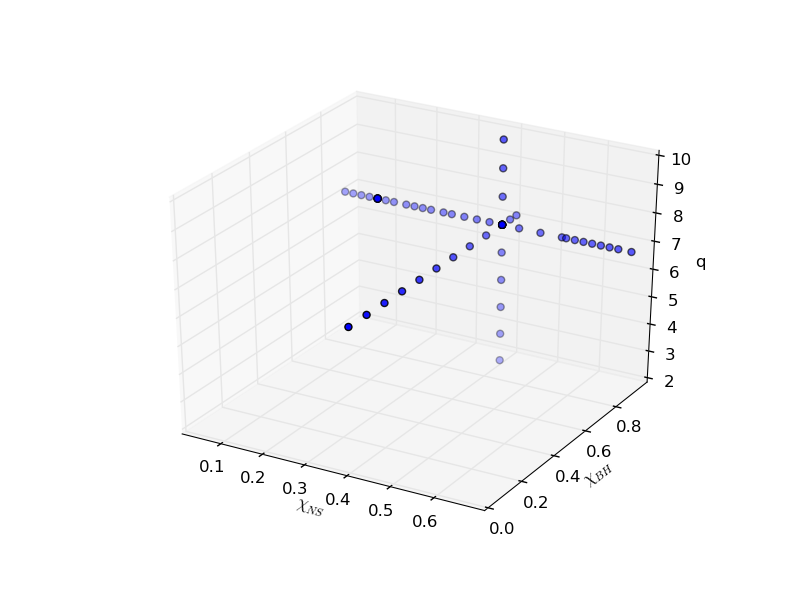
\includegraphics[width=0.95\columnwidth]{chap4/3dparam.png}
\caption[3d parameter space plot of Bh-Ns initial data sets.]{\label{fig:3dparam}
A parameter space scatter plot summarized where our sets of initial data have covered. The three axes are the magnitude of the black hole spin, the magnitude of the neutron star spin, and the mass ratio.}
\end{figure}

\subsection{Convergence of the Initial Data Solver}
To assess the convergence of the initial data solver we will begin by looking at the convergence of the iterative part of the solver. That is, the convergence of steps 1-10 in the iterative procedure
described above. To assess the convergence we will focus on one particular initial data set - namely the {\tt R14i60$\Uparrow$} initial data set. 

We begin by looking at the convergence of the Euler constant, $C$. In figure~\ref{Fig:EulerConv} we plot the absolute difference in $C$ between neighbouring iterations for the eight
different resolutions used in the initial data solve. In our notation, {\tt R1} is the first resolution, {\tt R2} is the second, etc. In the figure we see that at a given resolution these differences
seem to decrease exponentially with iteration. Meanwhile the differences also decrease with increasing resolution. This all shows that the initial data solver is working as it should. Note that although we've only shown
this plot for the {\tt R14i60$\Uparrow$} inital data set, we find similar results for all the other initial data sets we consider.


\begin{figure}
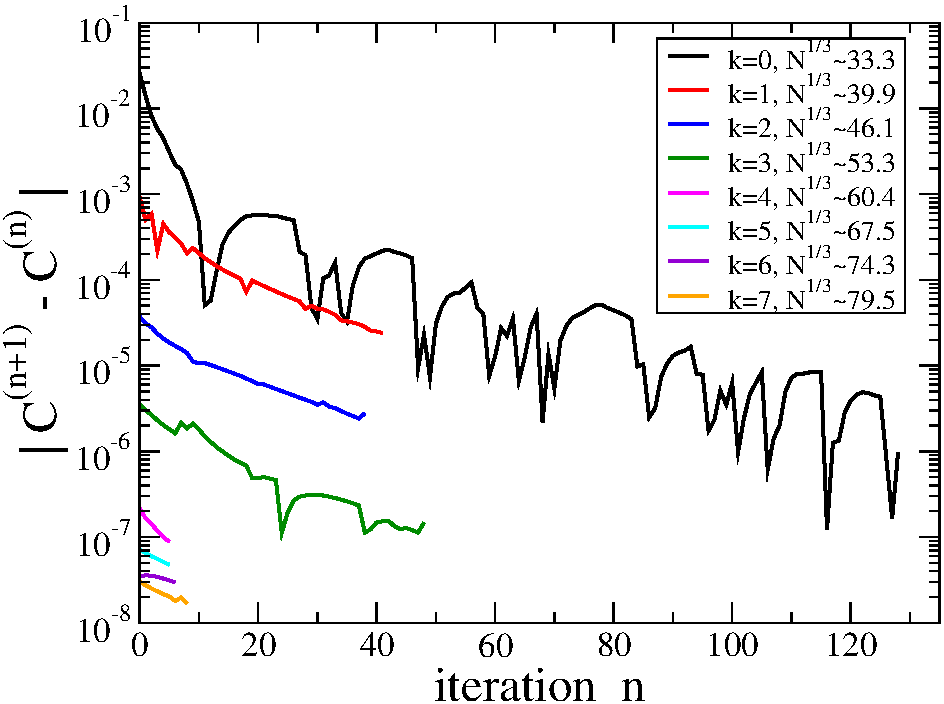
\includegraphics[width=0.95\columnwidth]{chap4/EulerConv}
\caption[Convergence of the Euler constant for the {\tt R14160$\Uparrow$}]{\label{Fig:EulerConv}
Absolute difference between neighbouring iterations of the Euler constant for the {\tt R14i160$\Uparrow$} initial data set. The eight curves {\tt R1}-{\tt R8} are the eight different resolutions
used in the initial data solve.}
\end{figure}

Next, we will look at the properties of the black hole to verify that they convergence as expected in the presence of a spinning neutron star. Again, we will focus on the {\tt R14i60$\Uparrow$} run, and look at the black hole spin parameter $a=J/M=M\chi$, which is controlled by the parameter $\Omega_j^{\rm BH}$ in Eq.~\ref{eq:BhBoundary3}. The target values are
\begin{eqnarray}
a&=&\chi_{\rm BH}M_{\rm BH}\\
&=&q\chi_{\rm BH}M_{\rm NS}^{\rm ADM}\\
a_x&=&q\chi_{\rm BH}(\sin60^{\circ})M_{\rm NS}^{\rm ADM}\\
a_z&=&q\chi_{\rm BH}(\cos60^{\circ})M_{\rm NS}^{\rm ADM}
\end{eqnarray}
We also look at the irreducible mass of the black hole, $M_{\rm irr}$. It is controlled by the size of the excision surface, and satisfies the relation
\begin{eqnarray}
M_{\rm BH}^{\rm irr}&=&\sqrt{\frac{A_{\rm AH}}{16\pi}}\\
(M_{\rm BH}^{\rm ADM})^2\left((M_{\rm BH}^{\rm irr})^2-\frac{a^2}{4}\right)&=&(M_{\rm BH}^{\rm irr})^4
\end{eqnarray}

In figure~\ref{Fig:BHSpinConv} we plot the fractional difference between the measured black hole spin and the target value, for both the x and z directions, as well as the fractional difference between
the measured black hole irreducible mass and the target value. The difference is plotted as a funciton of iteration, for four different resolutions. Note that the previous plot had eight different resolutions, while this one only has four. This is because the black hole spin is only computed for the first four resolutions - afterwards it is no longer solved for or measured. We note that in general we see a decrease in this difference with iteration, especially at the first resolution, therefore showing that the iterative solver is correctly driving the the black hole properties to the target values.
We also note that this difference decrease with resolution, and that we are able to achieve an accuracy of about $10^{-5}$ in the BH spin and mass.

\begin{figure}
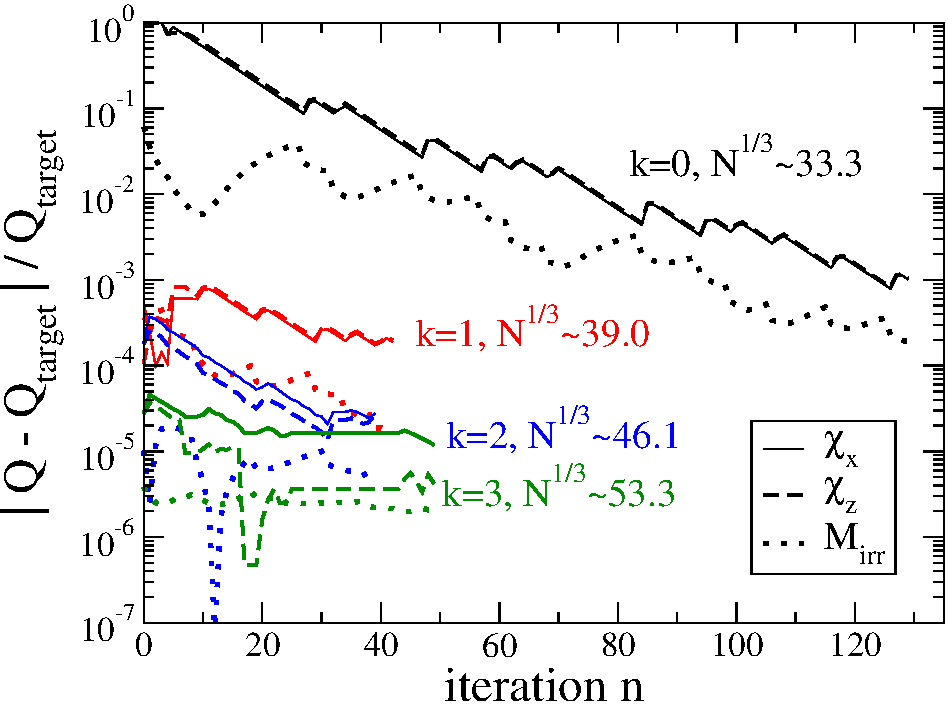
\includegraphics[width=0.95\columnwidth]{chap4/BHSpinConv}
\caption[Convergence of black hole spin and mass.]{\label{Fig:BHSpinConv} Plotted is the fractional difference from the target black hole spin and black hole mass in the {\tt R14i160$\Uparrow$} initial data set as a function of iteration. The four colours represent 
the four different resolutions at which the black hole spin is measured. The solid curves are for the $\hat{x}$ component of the BH spin, the dashed curves for the $\hat{z}$ component of the BH spin, and
the dotted curves are for the irreducible mass of the BH.}
\end{figure}

Having now established the convergence of the iterative procedure, we
turn now to establish the convergence with resolution of the global
properties of the solution, continuing to focus on the {\tt R14i160$\Uparrow$} ID set.

We begin by looking at the Hamiltonian and momentum constraints for the {\tt R14i160$\Uparrow$} initial data set.
The Hamiltonian constraint is computed as
\begin{equation}
H=||\frac{R_{\psi}}{8\psi^5}||
\end{equation}
where $R_{\psi}$ is the residual of Eq.~\ref{eq:XCTS-ConformalFactor}
and $||$ represents the $L2$ norm over the computational
domain. Similarly, the momentum constraint is computed as
\begin{equation}
M = ||\frac{R_{\beta}}{2\alpha\Psi^4}||
\end{equation}
where $R_{\beta}$ is the residual of Eq.~\ref{eq:XCTS-Shift}.
The constraints for this ID set are shown in figure~\ref{fig:HamMom}. We find exponential convergence in the constraints, as expected for spectral methods. The most notable feature
is that at {\rm R2} the constraints are higher than would be expected from the trend, otherwise. This is because the neutron star spin is only "turned on" at {\rm R2}, and so an additional amount of
solver time is needed to adjust to this change.
\begin{figure}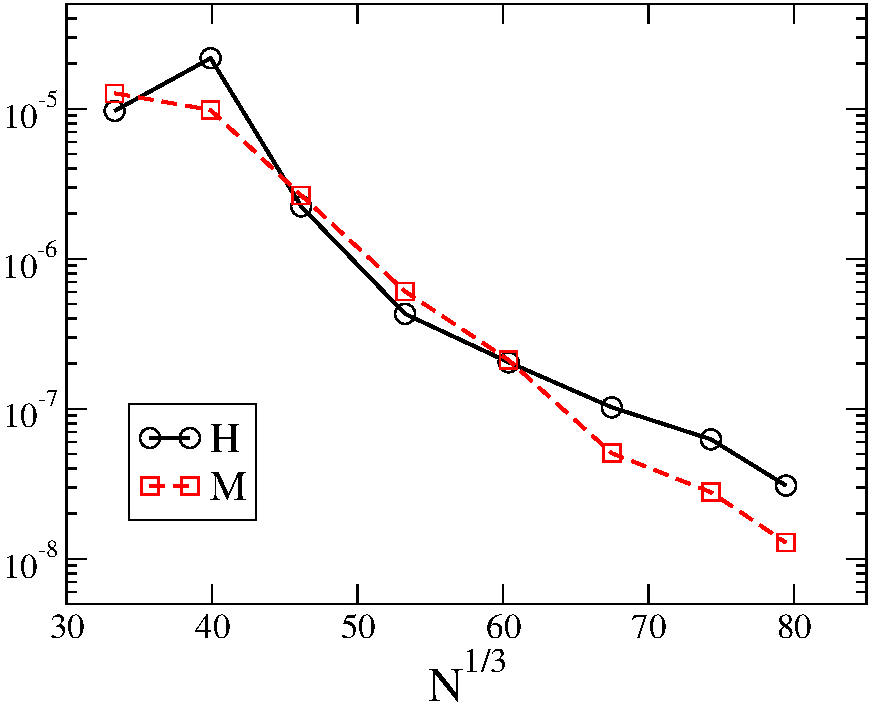
\includegraphics[width=0.95\columnwidth]{chap4/HamMom}
\caption[Hamiltonian and momentum constraints of the {\tt R14i160$\Uparrow$} ID set]{\label{fig:HamMom} The Hamiltonian and momentum constraints for the {\tt R14i160$\Uparrow$} initial data set
as a function of resolution. We find exponential convergence in both.}
\end{figure}

Finally, we look at the properties of the neutron star. As noted before,
the neutron star location is expressed as a sum of spherical
harmonics,
\begin{equation}
R(\theta,\phi)=\sum^{l_{\rm max}m_{\rm max}}_{l,m}c_{l,m}Y_{l,m}(\theta,\phi),
\end{equation}
where we generally use $l_{max}=11$.
To evaluate the convergence of the surface location, we define the
quantity,
\begin{equation}
\label{eq:NSSurf}
\Delta c(N)=\sqrt{\sum_{l,m}^{l_{\rm max}m_{\rm max}}\left(c_{lm}(N)-c^{*}_{lm}\right)^2}
\end{equation}
where $N$ represents the current resolution, and $*$ represents the
highest resolution. This quantity is plotted in
figure~\ref{fig:SpinDiff}. Note that similar to the black hole surface, the
neutron star surface is only computed for the first four resolution,
and so we have three data points shown. We do see exponential
convergence in this quantity. We also look at the convergence of the
neutron star spin $\chi_{\rm NS}$ measured at each resolution. In
figure~\ref{fig:SpinDif}, we plot the fractional difference in
$\chi_{\rm NS}$ between neighbouring resolutions, and find apparent
exponential convergence, although there are two disinctly different
slopes in the data, with the slope becoming more shallow at high
resolution. This is likely because we have stopped measuring the NS
surface at this point. However, we are able to measure the spin to an
accuracy of about $10^{-6}$. 
 We have ommited the first data point in this curve
because the neutron star spin is not turned on in the first
resolution, so by construction the first data point is artificially large.

\begin{figure}
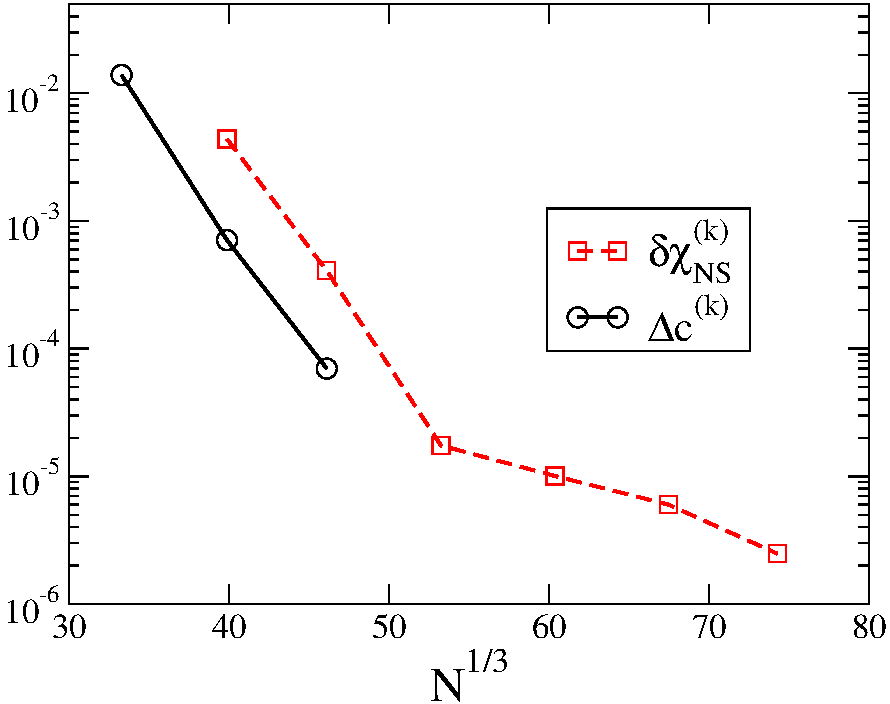
\includegraphics[width=0.95\columnwidth]{chap4/SpinDiff}
\caption[Neutron star surface and spin accuracy.]{\label{fig:SpinDiff}
  Accuracy of neutron star properties. Plotted are, as a function of resolution the accuracy of the computation of the neutron star
  surface, $\Delta c$, as defined in Eq.~\ref{eq:NSSurf} (black
  curve), and the fractional difference between neighbouring
  resolutions in the measured neutron star spin $\chi_{\rm NS}$ (red
  curve). This is for the {\tt R14i160$\Uparrow$} ID set.}
\end{figure}

The above data all show that we have established the convergence of
our initial data solver, by showing exponential convergence of the
iterative solver, the black hole properties, neutron star properties,
and the constraints.

\subsection{Other Initial Data Sequences}
We now turn to three more initial data sequences to help fill out the
bh-ns parameter space, as shown in Fig.~\ref{fig:3dparam}. We begin by
varying the neutron star spin from $\chi=0$ to $\chi\sim0.7$,
corresponding to $\omega_{\rm NS}\sim0.22$. The parameters in this
sequence are otherwise the same as in the {\tt R14i0} data sets
above, and the neutron star spin is kept aligned with the orbital
angular momentum. To demonstrate convergence, we begin by plotting the
Hamiltonian and momentum constraints for a subset of the generated
initial data sets, with $\chi\sim{0.1,0.3,0.5,0.7}$. This is shown in
Fig.~\ref{fig:OmegaSeqHamMom}. We note that in general we see
exponential convergence, as expected, but there are a few features
worth discussing in the data. The increase at {\tt R2}, as noted
earlier, is a monotonically increasing function of spin, as we might
expect. The larger the spin that gets turned on, the more difficult it
is for the solver to adjust. We also note that at high resolution, in
the $\chi\sim 0.7$ curve, we lose exponential convergence and the
curves flatten out around $10^{-6}$. This is likely a sign that the accuracy of the
solver is becoming limited, likely by approximations that go into the
solver. $\chi\sim 0.7$ is around the maximum theoretical neutron star
spin, so such difficulties may be expected.

\begin{figure}
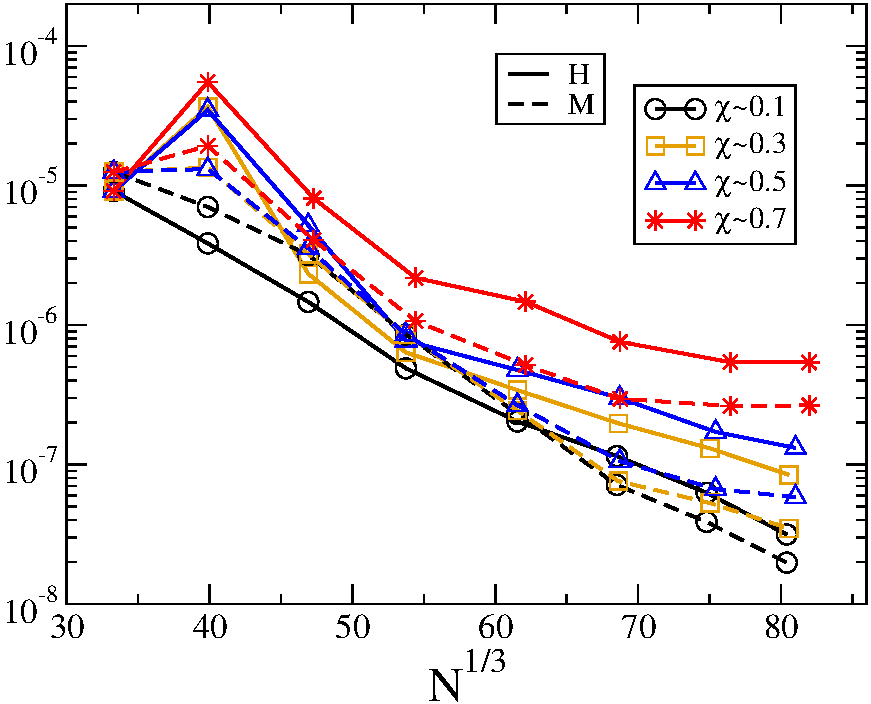
\includegraphics[width=0.95\columnwidth]{chap4/OmegaSeqHamMom}
\caption[Constraints for the $\chi_{\rm NS}$ sequence.]{\label{fig:OmegaSeqHamMom} Hamiltonian (solid curves) and
momentum (dotted curves) constraints for four different neutron star spins.}
\end{figure}

In Fig.~\ref{fig:ChiVOmega} we plot the full sequence, plotting the
measured neutron star spin $\chi_{\rm NS}$ as a function of the code
parameter $\omega_{\rm NS}$. As expected, we find a linear
relationship at low $\omega$, but the relationship becomes non-linear
at higher $\omega$, as the neutron star's size, and thus moment of
inertia, becomes an appreciable function of spin. We find that the
solver breaks down around $\chi_{\rm NS}\sim 0.7$ which is around the
theoretical maximum spin for $\Gamma=2$ polytropes. In
Fig.~\ref{fig:ChiVOmega} we have also plotted, in addition to this
bh-ns curve, a curve from ns-ns initial data sets. These data use
different NS parameters, with mass $M_{\rm ADM}=1.64M_{\odot}$ and
equation of state parameter $\kappa=123.6$. However, the curves remain
very close to each other in shape. Thus we see the neutron star spin
code seems to be working the same for the code described in this
chapter, as well as the code descriped in chapter \red{2}.

\begin{figure}
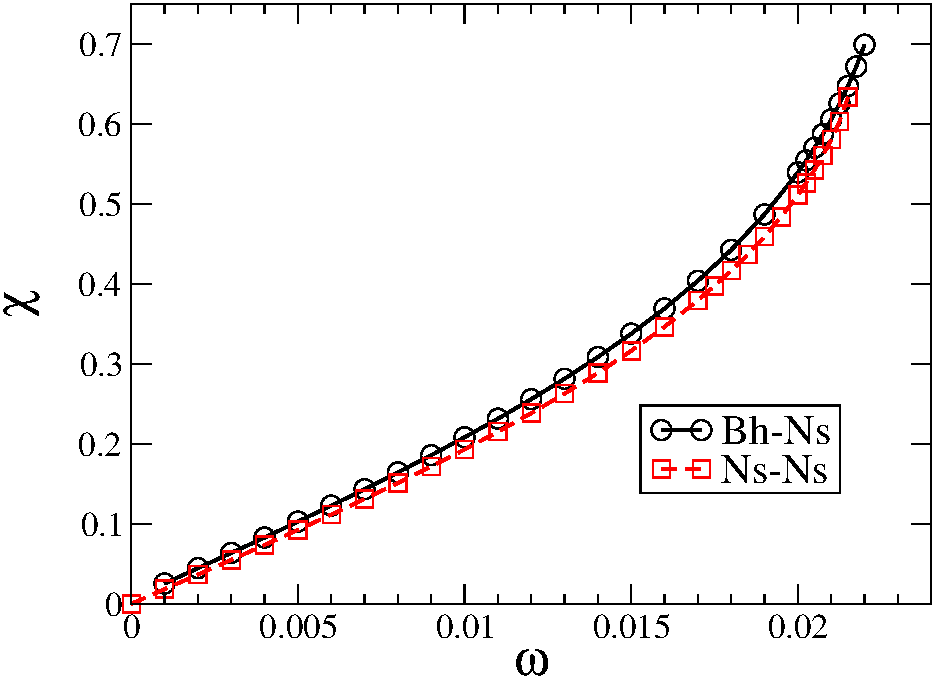
\includegraphics[width=0.95\columnwidth]{chap4/chiVOmega}
\caption[$\chi_{\rm NS}$ as a function of $\omega_{\rm NS}$ for bh-ns
binaries]
{\label{fig:ChiVOmega}
Neutron star spin $\chi$ as a function of neutron star spin parameter
$\omega$ for a sequence of initial data sets. The black hole spin is
constant at $\chi=0.9$ and the mass ratio is $q=7$. The red curve is
from ns-ns binaries, with somewhat different neutron star parameters.}
\end{figure}

After the sequence in $\chi_{\rm NS}$ we next look at a sequence in
$\chi_{\rm BH}$. In partiucar, we vary the black hole spin from
$\chi=0$ to $\chi=0.99$, keeping it aligned with the orbital angular
momentum.
 The other binary parameters are kept the same
as in the ${\tt R14i0\Uparrow}$ initial data set; that is $\chi_{\rm
  NS}\sim0.4$ and $q=7$. In Figs.~\ref{fig:chiSeqHam} and
~\ref{fig:chiSeqMom} we plot the Hamiltonian and momentum constraints,
respectively, for this sequence. We find exponential convergence in
all cases. It is interesting to note that the constraints seem to be
lowest at the highest black hole spins, $\chi_{\rm BH}=0.95$ and
$\chi_{\rm BH}=0.99$, while out might expect these to be the most
challenging cases.

\begin{figure}
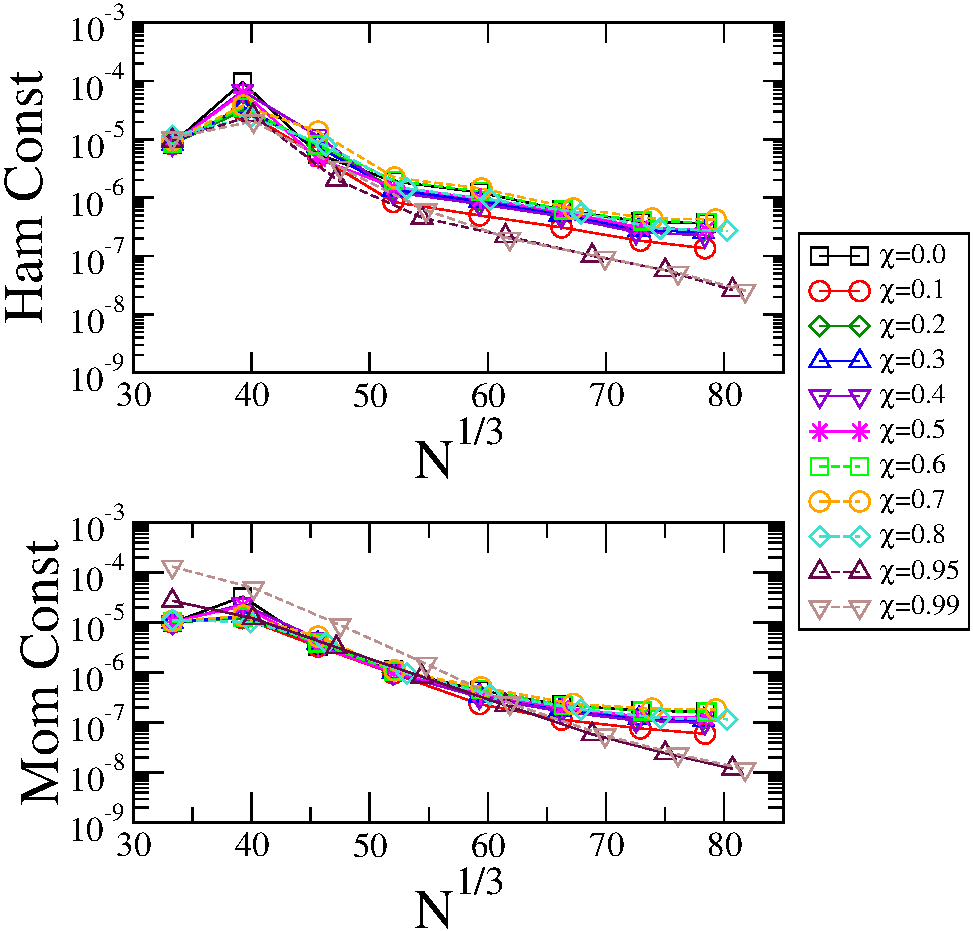
\includegraphics[width=0.95\columnwidth]{chap4/chiSeqHam}
\caption[Hamiltonian constraint for the sequence in $\chi_{\rm BH}$.]{\label{fig:chiSeqHam}Hamiltonian constraint versus
  resolution for our sequence of binaries where the black-hole spin is
  varied from $\chi_{\rm BH}=0$ to $\chi_{\rm BH}=0.99$. The neutron star spin is constant at $\chi_{\rm NS}\sim 0.4$ and the mass ratio is $q=7$. We find exponential convergence in all cases.}
\end{figure}

\begin{figure}
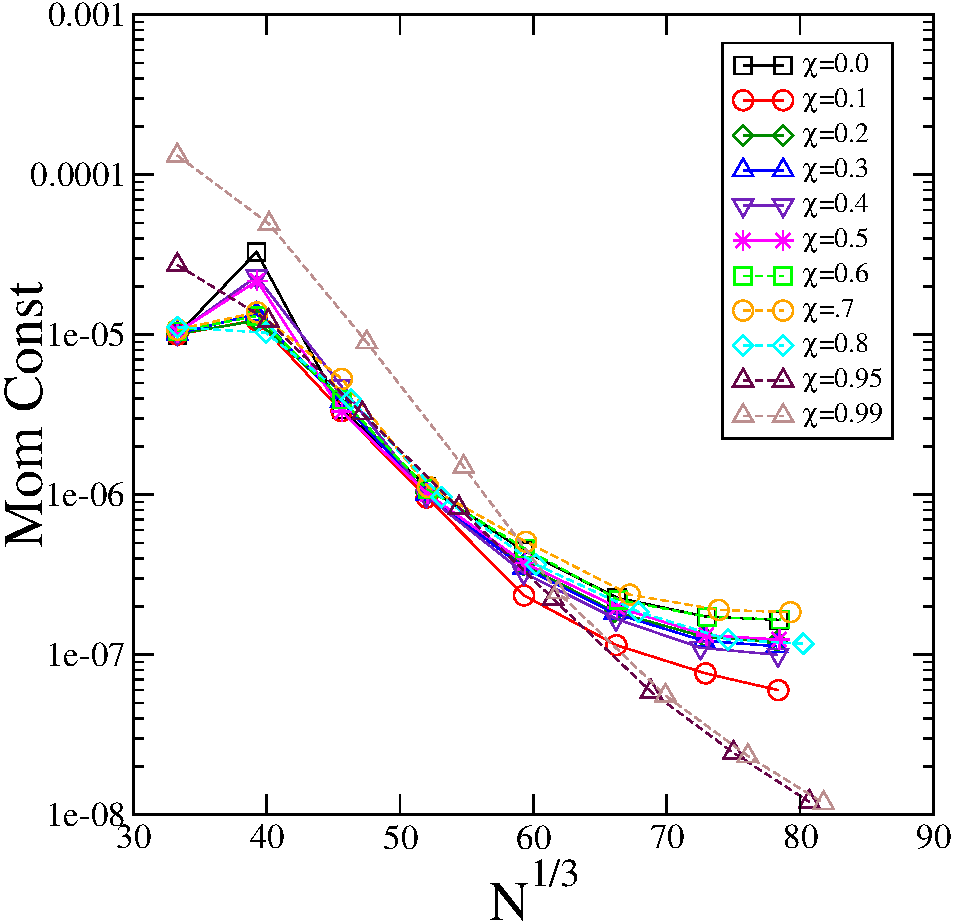
\includegraphics[width=0.95\columnwidth]{chap4/chiSeqMom}
\caption[Momentum constraints for the sequence in $\chi_{\rm BH}$.]{\label{fig:chiSeqMom} Same as
  Fig.~\ref{fig:chiSeqHam} but for the momentum constraint.}
\end{figure}

Since in this work we are largely concerned with neutron star spin, it
is interesting to consider how the measured neutron star spin,
$\chi_{\rm NS}$ couples to other binary parameters. To lowest order,
it should depend only on $\omega_{\rm NS}$, but in practice in may
also depend on the parameters of the black hole. For this sequence in
$\chi_{\rm BH}$, we plot $\chi_{\rm NS}$ as a function of $\chi_{\rm
  BH}$ in figure~ref\{fig:chichi}. There is a clear negative slope in
this plot. \red{I am not sure how to explain this!}
\red{Currently testing how NS spin direction couples.}
\red{Should also test how BH spin direction couples.}

\begin{figure}
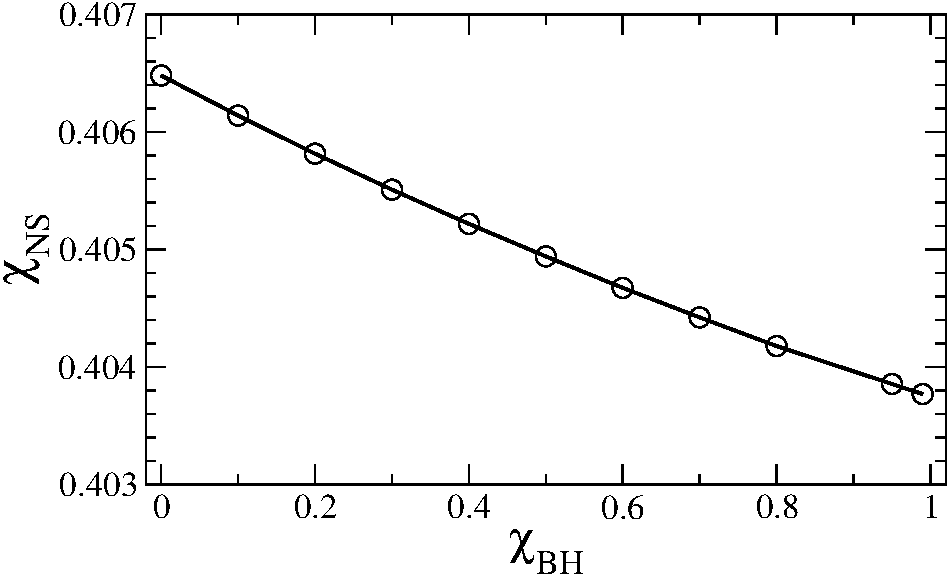
\includegraphics[width=0.95\columnwidth]{chap4/chichi}
\caption[\red{add}]{\label{fig:chichi}Neutron star spin $\chi_{\rm NS}$ as a fucntion of black hole spin $\chi_{\rm BH}$ for this sequence. We notice a small but significant downward linear trend. \red{Can we explain this?}}
\end{figure}




Finally, we consider a sequence where we vary the mass ratio from
$q=2$ to $q=10$. In this sequence we keep the other binary parameters
the same as in the ${\tt R14i0\Uparrow}$ initial data set. In this sequence, we keep the
orbtial parameters $M\Omega$ and $D/M$ constant. As discussed above,
we expect that this will induce a eccentricity of a few percent. To
assess convergence, we plot the Hamiltonian and momentum constraints
for this sequence in Figs.~\ref{fig:qSeqHam} and
~\ref{fig:qSeqMom}. We find exponential convergence in all
cases. Interestingly, no clear pattern in $q$-space emerges.

\begin{figure}
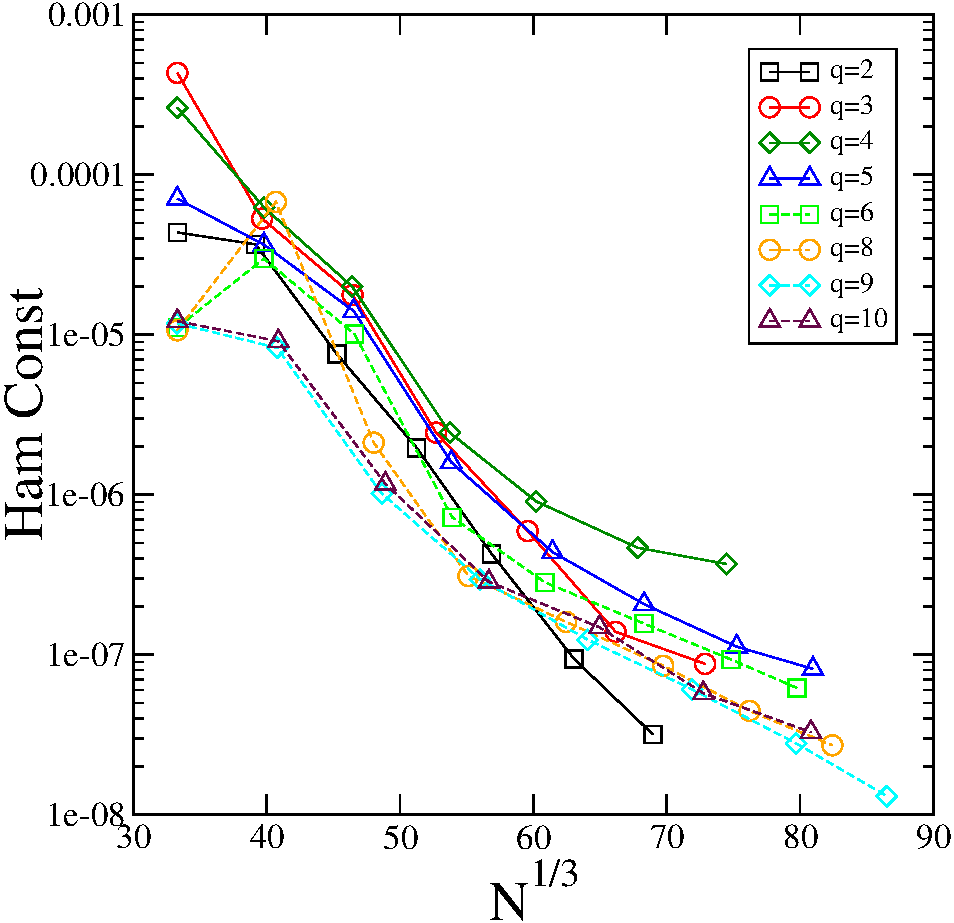
\includegraphics[width=0.95\columnwidth]{chap4/qSeqHam}
\caption[Hamiltonian constraint for the $q$ sequence.]{\label{fig:qSeqHam}Hamiltonian constraint versus resolution for our sequence of binaries where the mass ratio is varied from $q=2$ up to $q=10$. The neutron star spin is constant at $\chi_{\rm NS}\sim 0.4$ and the black hole spin is $\chi_{\rm BH}=0.9$. We find exponential convergence, as expected, in all cases.}
\end{figure}

\begin{figure}
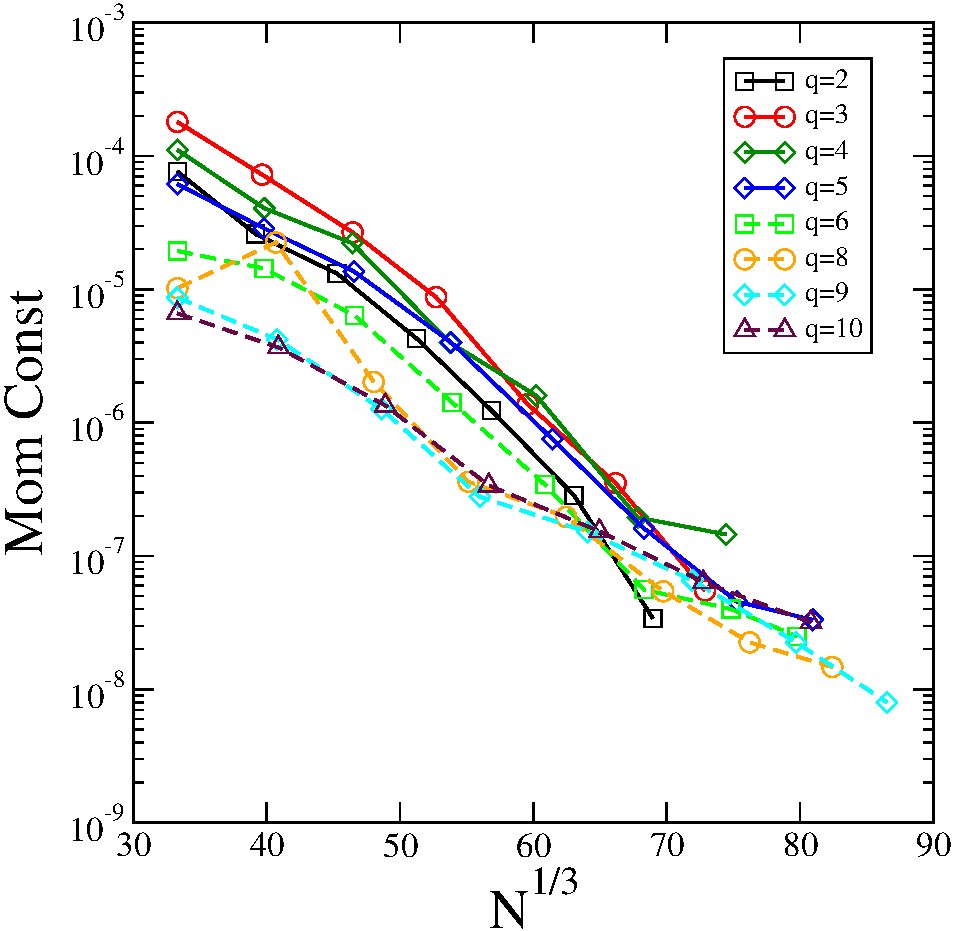
\includegraphics[width=0.95\columnwidth]{chap4/qSeqMom}
\caption[Momentum constraint for the $q$ sequence.]{\label{fig:qSeqMom} Same as Fig.~\ref{fig:qSeqHam}
  but for the momentum constraint.}
\end{figure}

As with the previous sequence, it is interesting to look at the
properties of $\chi_{\rm NS}$ as a function of $q$. This is shown in
Fig~\ref{fig:qchi}. Although there is not a great amount of variation,
apart from $q=2$, there is a clear trend of
$\chi_{\rm NS}$ decreasing with $q$. \red{can we explain this?}
\red{what tests to do?}
\begin{figure}
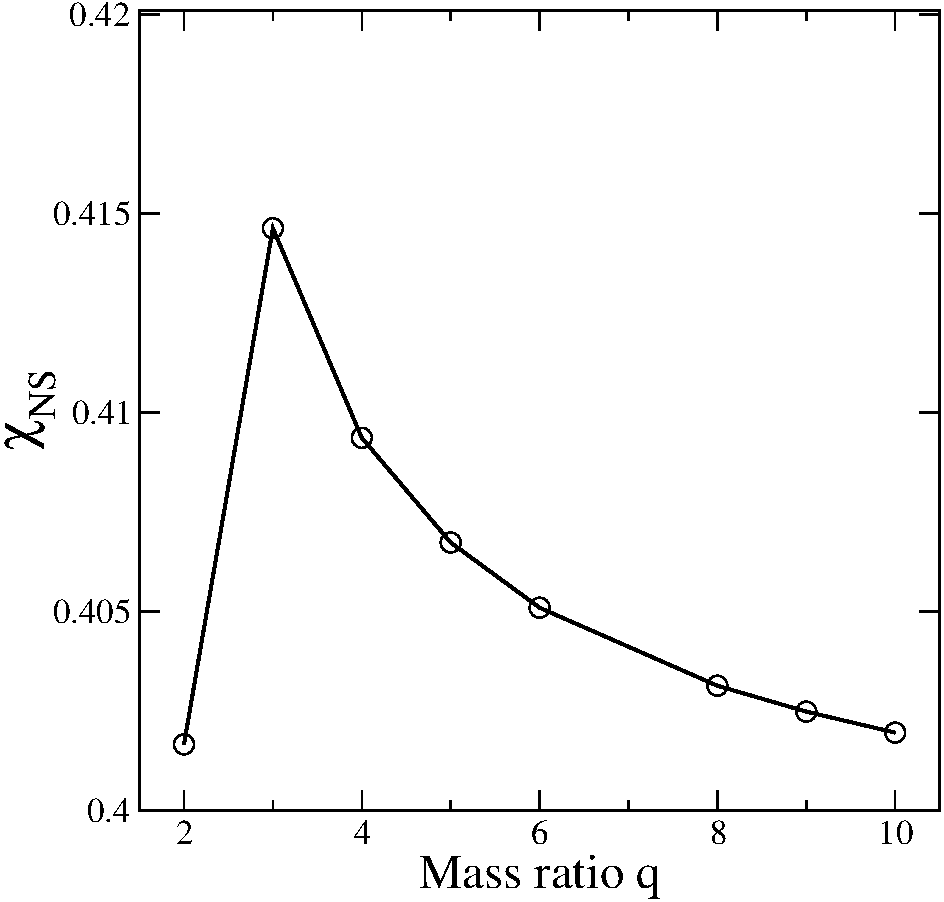
\includegraphics[width=0.95\columnwidth]{chap4/qchi}
\caption[$\chi_{\rm NS}$ as a function of mass ratio $q$.]{\label{fig:qchi}Neutron star spin $\chi_{\rm
    NS}$ as a function of mass ratio $q$ for this sequence. We notice
  a downward trend for $q \geq 3$. \red{Can we explain this?}}
\end{figure}



%\section{Comparison with Black-Hole Binaries}
%Comparison

\section{Conclusion}
Concluding remarks
